% Metaboenrich: Ohm's-law current flow on the metabolite-reaction network
% Compiles on Overleaf with pdfLaTeX (standard packages only).
\documentclass[11pt]{article}

\usepackage[margin=1in]{geometry}
\usepackage[T1]{fontenc}
\usepackage{lmodern}
\usepackage{amsmath,amssymb,amsthm}
\usepackage{booktabs}
\usepackage{tabularx}
\usepackage{enumitem}
\usepackage{xcolor}
\usepackage{tikz}
\usetikzlibrary{arrows.meta,positioning}
\usepackage[colorlinks=true,linkcolor=blue!50!black,urlcolor=blue!50!black,citecolor=blue!50!black]{hyperref}

\newcommand{\code}[1]{\texttt{#1}}
\newcommand{\R}{\mathbb{R}}
\newcommand{\Reff}{R_{\mathrm{eff}}}
\newtheorem*{remark}{Remark}

\title{Metaboenrich step 5 (default):\\
Ohm's-law current flow on the metabolite--reaction network}
\author{Metaboenrich methods note}
\date{Code reference: \code{metaboenrich/flow.py}, commit \code{0f6c135} (branch \code{directed-rw})}

\begin{document}
\maketitle

\begin{abstract}
Metaboenrich ranks genes, reactions and pathways from a differential metabolite
abundance (DAA) table. Its default scoring step treats the metabolic network as an
electrical circuit. Every metabolite that went up is a current source and every
metabolite that went down is a sink. For each source--sink pair, one unit of current
is injected and Kirchhoff's and Ohm's laws give the current on every edge. Reactions
that carry a large share of the current, or that are the only route for some pair,
rank high. This note defines the method exactly as implemented, shows how it is
solved efficiently, and lists its properties and limits. A companion note describes
the experimental alternative, a directed absorbing random walk.
\end{abstract}

\tableofcontents

%======================================================================
\section{Where this step sits in the pipeline}
%======================================================================

The main run (\code{python -m metaboenrich}) has seven steps:
\begin{enumerate}[nosep]
  \item load Human-GEM v2.0.1 (\code{gem.py});
  \item decide which metabolites are currency (\code{network.py});
  \item map the DAA table onto model metabolites (\code{daa.py});
  \item build the metabolite--reaction graph (\code{network.py});
  \item \textbf{solve the current flow} (\code{flow.py}, this note);
  \item score and rank reactions, genes and pathways (\code{scoring.py});
  \item write the outputs (\code{\_\_main\_\_.py}, \code{cytoscape.py}).
\end{enumerate}
Step 5 takes the graph from step 4 and the source and target lists from step 3, and
returns per-node and per-edge arrays (a \code{FlowResult}) that step 6 turns into
ranked tables. It corresponds to protocol \S1.4 (current flow) and \S2.2 (directed
pair filter).

%======================================================================
\section{The network as a circuit}
%======================================================================

\subsection{Graph}
The graph $G=(V,E)$ is bipartite. $V = M \cup R$ holds one node per metabolite
(compartments merged) and one node per reaction. An edge joins a metabolite to a
reaction it takes part in, as substrate or product. Currency metabolites (H$^+$,
H$_2$O, phosphate, cofactor exchange pairs such as ATP/ADP, \dots) are removed
before the graph is built, so they cannot act as shortcuts. On Human-GEM the locked
network has $3{,}958$ metabolites, $6{,}377$ reactions and $16{,}356$ edges.

Every edge has unit conductance (resistance $1\,\Omega$). Edges are
\emph{undirected}: reaction directions are not used in the electrical problem.

\subsection{Incidence matrix and Laplacian}
Number the edges $e=1,\dots,m$ and the nodes $v=1,\dots,n$. The signed incidence
matrix $B\in\R^{m\times n}$ has, for edge $e=(\mu,\rho)$ joining metabolite $\mu$
and reaction $\rho$,
\[
  B_{e\mu} = +1,\qquad B_{e\rho} = -1,\qquad B_{ev}=0 \text{ otherwise.}
\]
The orientation is a bookkeeping convention: a positive edge current means current
flows from the metabolite into the reaction. The weighted graph Laplacian with unit
conductances is
\[
  L = B^{\top}B \in \R^{n\times n}.
\]
$L$ is symmetric and positive semi-definite. Its null space is spanned by the
indicator vectors of the connected components, so $L$ is singular.

%======================================================================
\section{One source--target pair}
%======================================================================

\subsection{Kirchhoff and Ohm}
For a source $s$ (log$_2$FC $>0$) and a target $t$ (log$_2$FC $<0$) in the same
connected component, inject one ampere at $s$ and withdraw it at $t$:
\begin{equation}
  L\,x^{st} = b^{st},\qquad b^{st} = e_s - e_t,
  \label{eq:kirchhoff}
\end{equation}
where $x^{st}\in\R^n$ are the node potentials and $e_v$ is the $v$-th unit vector.
Ohm's law gives the edge currents
\begin{equation}
  I^{st} = B\,x^{st}\in\R^{m},
  \qquad I^{st}_e = x^{st}_\mu - x^{st}_\rho \text{ for } e=(\mu,\rho).
  \label{eq:ohm}
\end{equation}
Kirchhoff's current law holds by construction, $B^{\top}I^{st} = b^{st}$: one unit
leaves $s$, one unit arrives at $t$, and current is conserved at every other node.

\subsection{Throughput}
The throughput of node $v$ for the pair $(s,t)$ is the current passing through it,
\begin{equation}
  T^{st}(v) = \tfrac12 \sum_{e\ni v} \bigl|I^{st}_e\bigr|
  \quad (v\neq s,t),
  \qquad T^{st}(s)=T^{st}(t)=0 .
  \label{eq:throughput}
\end{equation}
The factor $\tfrac12$ counts current once: what enters an intermediate node also
leaves it. $T^{st}(v)\in[0,1]$, and $T^{st}(v)=1$ means every path from $s$ to $t$
passes through $v$ (a bottleneck). The endpoints are set to zero because they
trivially carry the whole unit. This is the current-flow betweenness of
Newman (2005) and Brandes and Fleischer (2005), restricted to the measured pairs.

\subsection{Effective resistance}
The potential drop between the endpoints is the effective resistance,
\[
  \Reff(s,t) = x^{st}_s - x^{st}_t ,
\]
small when $s$ and $t$ are joined by many short, parallel routes. For each source
or target the output reports the mean effective conductance $1/\Reff$ over its pairs
(\code{eff\_conductance}) and the mean largest current on any one of its own edges
(\code{max\_edge\_share}), which shows whether its current leaves through a single
reaction.

\begin{figure}[ht]
\centering
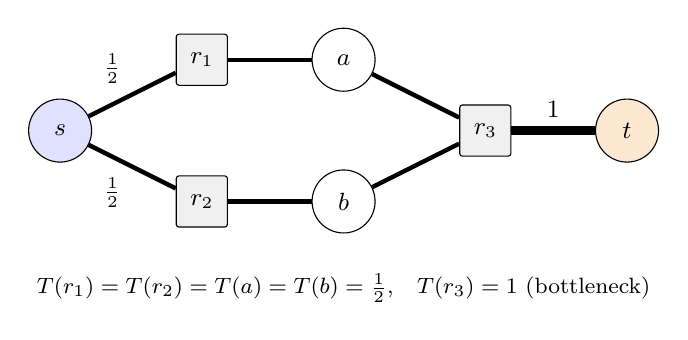
\begin{tikzpicture}[
  met/.style={circle,draw,minimum size=8mm,inner sep=0pt},
  rxn/.style={rectangle,draw,rounded corners=1pt,minimum size=6.5mm,inner sep=0pt,fill=black!6},
  every node/.style={font=\small}]
  \node[met,fill=blue!12] (s) at (0,0) {$s$};
  \node[rxn] (r1) at (1.8,0.9) {$r_1$};
  \node[rxn] (r2) at (1.8,-0.9) {$r_2$};
  \node[met] (a) at (3.6,0.9) {$a$};
  \node[met] (b) at (3.6,-0.9) {$b$};
  \node[rxn] (r3) at (5.4,0) {$r_3$};
  \node[met,fill=orange!18] (t) at (7.2,0) {$t$};
  \draw[line width=1.6pt] (s)--(r1) node[midway,above left] {$\tfrac12$};
  \draw[line width=1.6pt] (s)--(r2) node[midway,below left] {$\tfrac12$};
  \draw[line width=1.6pt] (r1)--(a);
  \draw[line width=1.6pt] (r2)--(b);
  \draw[line width=1.6pt] (a)--(r3);
  \draw[line width=1.6pt] (b)--(r3);
  \draw[line width=3pt] (r3)--(t) node[midway,above] {$1$};
  \node[align=center,font=\footnotesize] at (3.6,-2.0)
    {$T(r_1)=T(r_2)=T(a)=T(b)=\tfrac12$,\quad $T(r_3)=1$ (bottleneck)};
\end{tikzpicture}
\caption{Current splits over parallel routes and recombines. Reaction $r_3$ is the
only way into $t$, so it carries the full unit: bottleneck $=1$.}
\label{fig:split}
\end{figure}

%======================================================================
\section{All pairs at once: grounding and one factorisation}
%======================================================================

Solving \eqref{eq:kirchhoff} separately for all $|S|\times|T|$ pairs, or forming the
pseudoinverse $L^{+}$ (dense, $O(n^3)$), would be wasteful. The implementation uses
linearity instead.

\paragraph{Grounding.} In each connected component $C$, fix the potential of its
first node $g_C$ to zero. Deleting that row and column gives a non-singular matrix
$L_C$. Grounding shifts all potentials by a constant, which leaves edge currents and
effective resistances unchanged.

\paragraph{Unit solves.} For each source or target $v$ in $C$, solve once
\begin{equation}
  L_C\, y^{v} = e_v ,
  \label{eq:unit}
\end{equation}
the potentials when one unit enters at $v$ and leaves at the ground. Each component
is LU-factorised once (\code{scipy.sparse.linalg.splu}) and reused for all its
right-hand sides.

\paragraph{Pairs by subtraction.} For any pair in $C$,
\[
  x^{st} = y^{s} - y^{t},
\]
because the right-hand sides subtract to $e_s - e_t$ and the ground terms cancel.
So $|S|+|T|$ solves cover all $|S|\,|T|$ pairs. Pairs are then processed in blocks
of 128: $I = B X$ and $T=\tfrac12|B|^{\top}|I|$ are sparse--dense products.

%======================================================================
\section{Combining pairs into scores}
%======================================================================

Let $P$ be the retained pairs and $w_{st}$ the pair weights. By default every pair
has $w_{st}=1$ (one ampere per pair, as in the protocol). With
\code{--pair-weight fc}, $w_{st} = \tfrac12(\varphi_s+\varphi_t)$ with
$\varphi_v = |\log_2\mathrm{FC}_v|$. With $W=\sum_{P} w_{st}$:

\begin{align}
  \text{accumulated current}\quad A(v) &= \textstyle\sum_{(s,t)\in P} w_{st}\,T^{st}(v),\\
  \text{conductivity}\quad c(v) &= A(v)/W,\\
  \text{bottleneck}\quad \beta(v) &= \max_{(s,t)\in P} T^{st}(v),\\
  \text{bottleneck fraction}\quad f_\tau(v) &= \tfrac{1}{W}\textstyle\sum_{P} w_{st}\,\mathbf 1\!\left[T^{st}(v)\ge\tau\right],\quad \tau=0.5,\\
  \text{edge current}\quad \bar I_e &= \tfrac1W\textstyle\sum_P w_{st}\,|I^{st}_e|,\qquad I^{\max}_e = \max_P |I^{st}_e| .
\end{align}

Conductivity is the share of the total current that passes through $v$; the
bottleneck is the largest share for any single pair.

\subsection{Leave-one-out scores}
A reaction can score highly only because one measured metabolite has a single way
out. The leave-one-out scores ask whether the score survives dropping any one
metabolite. For a source $k$, let $A_k(v)$ and $W_k$ be the sums over the pairs that
use $k$, and $\beta_k(v)$ the maximum over those pairs. A metabolite is
\emph{droppable} if $0 < W_k < W$ (dropping it leaves some pairs). Then
\[
  c^{\mathrm{loo}}(v) = \min_{k\ \mathrm{droppable}} \frac{A(v)-A_k(v)}{W-W_k},
\]
taken over droppable sources and targets alike, and clipped at $0$. The leave-one-out
bottleneck is the second-largest of the per-metabolite maxima $\beta_k(v)$, the worst
case after dropping the metabolite with the largest one. If nothing is droppable (one
source and one target), the raw values are used. Raw scores are the default
(\code{--scoring raw}); \code{--scoring loo} ranks on these columns instead.

%======================================================================
\section{Variants}
%======================================================================

\paragraph{Pair exclusion.} Pairs in different connected components cannot carry
current and are written to \code{excluded\_pairs.tsv} (``disconnected'').

\paragraph{Directed mode (\code{--mode directed}, protocol \S2.2).} Pairs with no
directed path $s\to t$ along reaction directions are also excluded. This is
\emph{only} a filter: the remaining pairs are solved on the same undirected
Laplacian, so current can still run against a reaction's direction. Directed
current (protocol \S2.3) is not implemented; the directed absorbing random walk is
the experimental alternative.

\paragraph{One-sided data (\code{--one-sided auto}).} If only increases (or only
decreases) are significant, the measured but unchanged metabolites form a ground set
$\mathcal G$. Each source injects one unit withdrawn evenly across the ground nodes
in its component,
\[
  b = e_s - \tfrac{1}{|\mathcal G_C|}\textstyle\sum_{g\in\mathcal G_C} e_g ,
\]
and symmetrically when only targets exist. Ground nodes are sinks and are not scored.

%======================================================================
\section{From node scores to ranked genes and pathways}
%======================================================================
Step 6 is shared with the random walk.
\begin{itemize}[nosep]
  \item Reactions with $c>0$ get a final score: the mean of the percentile ranks of
        conductivity and bottleneck (raw or leave-one-out).
  \item A gene takes the best final score among the reactions it catalyses
        (gene--protein--reaction and/or logic is ignored).
  \item Pathways (Human-GEM subsystems) are tested for over-representation among the
        top 100 reactions with a hypergeometric test against all network reactions,
        with Benjamini--Hochberg correction.
  \item The Cytoscape subnetwork keeps edges with $I^{\max}_e\ge 0.1$.
\end{itemize}

%======================================================================
\section{Properties and limits}
%======================================================================
\begin{itemize}
  \item \textbf{Direction-blind.} The circuit is undirected, so current can run
        through an irreversible reaction backwards.
  \item \textbf{Co-substrate hops.} Current can enter a reaction through one
        substrate and leave through another (for $A+B\to C$, the route
        $A\to r\to B$), a step no enzyme performs. Currency removal limits the worst
        cases but does not prevent this in general.
  \item \textbf{Every pair counts equally} by default; fold change enters only
        through \code{--pair-weight fc}, and only as a pair weight, not in
        $Lx=b$.
  \item \textbf{Bounded and interpretable.} Throughput lies in $[0,1]$; a value of
        $1$ is a cut vertex for that pair.
  \item \textbf{Global.} Current spreads over every parallel route, so long
        alternative routes still receive some current. This makes the method
        robust to single missing reactions, but dilutes the signal in dense
        regions.
  \item \textbf{Exact and fast.} One sparse LU per component; the full run on
        Human-GEM takes a few seconds.
\end{itemize}

\begin{remark}[Link to random walks]
On an undirected graph, the unit current from $s$ to $t$ equals the expected net
number of times a simple random walker started at $s$ and stopped at $t$ crosses each
edge (Newman, 2005). Current flow is therefore already a random-walk method, on an
undirected graph, one pair at a time, with every step equally likely. The directed
absorbing random walk changes exactly those three things.
\end{remark}

%======================================================================
\section{Benchmark}
%======================================================================
Inborn errors of metabolism (plasma $z$-scores from Thistlethwaite et al.\ 2020 and
Miller et al.\ 2015): rank of the known causal gene among the $2{,}302$ network genes,
raw scoring; lower is better. Source: \code{docs/decisions.md}, D17.

\begin{center}
\begin{tabular}{@{}llrr@{}}
\toprule
Level & Measure & Current flow & Absorbing walk\\
\midrule
Group (20 primary disorders) & median rank & 88.5 & 48\\
 & in top 100 & 11 & 13\\
 & in top 10 & 3 & 5\\
Patient (159 primary patients) & median rank & 134 & 67\\
 & in top 100 & 47\% & 55\%\\
 & in top 10 & 5\% & 28\%\\
\bottomrule
\end{tabular}
\end{center}
Current flow remains the default: the blind predictions on published datasets (D14)
were made with it, and the walk's gains come from one benchmark.

%======================================================================
\section{Implementation map}
%======================================================================
\begin{center}
\small
\begin{tabularx}{\linewidth}{@{}lX@{}}
\toprule
Code (\code{metaboenrich/}) & What it computes\\
\midrule
\code{network.Graph.incidence()} & $B$; $L=B^{\top}B$\\
\code{network.Graph.components()} & connected components (grounding, pair filter)\\
\code{flow.select\_pairs()} & retained and excluded pairs; directed filter\\
\code{flow.\_potentials()} & grounded LU per component, unit solves \eqref{eq:unit}\\
\code{flow.current\_flow()} & $I=BX$, throughput \eqref{eq:throughput}, $A$, $c$, $\beta$, $f_\tau$, edge currents, $\Reff$\\
\code{flow.\_leave\_one\_out()} & $c^{\mathrm{loo}}$, $\beta^{\mathrm{loo}}$\\
\code{scoring.reaction\_table()} & final score from percentile ranks\\
\code{scoring.gene\_table()}, \code{pathway\_table()} & gene ranking; pathway enrichment\\
\bottomrule
\end{tabularx}
\end{center}

\section*{References}
\begin{itemize}[nosep,leftmargin=*]
  \item Newman, M.\,E.\,J. (2005). A measure of betweenness centrality based on random
        walks. \emph{Social Networks} 27, 39--54.
  \item Brandes, U.\ and Fleischer, D. (2005). Centrality measures based on current
        flow. \emph{STACS 2005}, LNCS 3404, 533--544.
  \item Doyle, P.\,G.\ and Snell, J.\,L. (1984). \emph{Random Walks and Electric
        Networks}. Mathematical Association of America.
  \item Metaboenrich protocol, \S1.4 and \S2.2 (\code{Metaboenrich-Protocol.pdf}).
\end{itemize}

\end{document}
